% Provenance (never printed): old seconde/premiere S material on the
% atmosphere (storms, cyclones, the energy of the water cycle) and the
% natural-hazard themes of SVT; see sources/book2/PROVENANCE.md. Tracks,
% genesis statistics and the pressure--wind relation are computed in
% figdata/grade-10/cyclones.py from IBTrACS v04r01; the surge, thunder and
% energy numbers in the same script.
\chapter{风暴与热带气旋}\label{ch:g10:storms-and-cyclones}

炎热的夏日午后，一场风暴来临。天色变暗，一阵冷风
扫过街道，一道\omterm{def:g10:storms-and-cyclones:lightning}{闪电}照亮了云层——你开始数数：
一、二、三、\ldots{}，九秒后雷声滚滚而来。风暴距离你
约 3 千米。一小时后风暴便会过去，空气凉爽清新。在温暖的热带海洋上，
同样的条件——温暖潮湿、上升并凝结的空气——
能够组织成另一种规模的风暴：\omterm{def:g10:storms-and-cyclones:tropical-cyclone}{热带气旋}，
直径达数百千米，可持续数天，风力足以摧毁森林，
并使海面上升，淹没整片海岸。本章讨论
\omterm{def:g10:storms-and-cyclones:thunderstorm}{雷暴}、\omterm{def:g10:storms-and-cyclones:tornado}{龙卷风}和\omterm{def:g10:storms-and-cyclones:tropical-cyclone}{热带气旋}，
以及它们的能量
从何而来。

\begin{safety}
若听到雷声，\omterm{def:g10:storms-and-cyclones:lightning}{闪电}就可能击中你。
应进入建筑物或封闭的汽车内，并待在其中，直到最后一次雷声过后很久。
切勿在孤立的树下躲避，远离山顶、空旷的田野和水域。
\end{safety}

\begin{recall}
气团、锋、低压（低气压区）和反气旋
在天气图上用等压线标出，等压线即气压相等的线（第 1 册，八年级）。
自然危害是可能伤害人类及其建造物的自然事件（第 1 册，五年级）。
声音在空气中传播的速度约为
\qty{340}{m/s}，光几乎瞬间到达（物理类教材）。温暖潮湿的空气
上升时冷却，在\omterm{def:g10:why-clouds-form:condensation-level}{凝结高度}形成云，并释放\omterm{def:g10:earth-energy-budget:latent-heat}{潜热}；
\omterm{def:g10:why-clouds-form:humidity}{饱和}空气往往是不稳定的
（见\cref{ch:g10:why-clouds-form}）。
\end{recall}

\section{雷暴}

\begin{definition}[雷暴]\label{def:g10:storms-and-cyclones:thunderstorm}
称\emph{雷暴}\index{雷暴}为由
积雨云产生的风暴，伴有\omterm{def:g10:storms-and-cyclones:lightning}{闪电}和雷声，通常有强降水，
并伴随阵风，有时还有冰雹。
\end{definition}

\omterm{def:g10:storms-and-cyclones:thunderstorm}{雷暴}由不稳定的潮湿空气发展而来。第一阶段，积云
在强上升气流的带动下向上生长；凝结释放\omterm{def:g10:earth-energy-budget:latent-heat}{潜热}，
使上升空气比周围空气更暖。成熟阶段，云顶伸入
上方稳定的空气层并向外铺展成砧状云；
雨滴和冰雹长大到足以下落，降水拖着冷空气一同下沉，
形成下沉气流，在地面向外扩散，形成冷阵风锋。
消散阶段，下沉气流控制整个云体，
切断暖湿空气的供应，
风暴靠降水把自身耗尽。

\begin{omfigure}
\begin{tikzpicture}[font=\footnotesize, >={Stealth[length=2mm]}]
  \foreach \dx/\title in {0/{1. 发展阶段}, 4.6/{2. 成熟阶段}, 9.2/{3. 消散阶段}}
    \node[anchor=north] at (\dx+1.6,-0.15) {\title};
  \draw[thick, black!60] (-0.3,0) -- (12.9,0);
  % stage 1: a tall cumulus
  \pic[scale=1.4, transform shape] at (1.6,1.2) {puffycloud};
  \pic[scale=1.1, transform shape] at (1.6,2.0) {puffycloud};
  \foreach \x in {1.2,1.6,2.0} \draw[->, thick, omThm!80!black] (\x,0.2) -- (\x,2.6);
  % stage 2: cumulonimbus with anvil
  \fill[black!8, draw=black!50] (5.0,1.0) -- (4.9,4.0) -- (4.2,4.4) -- (8.0,4.6) -- (7.4,4.0) -- (7.2,1.0) -- cycle;
  \draw[->, thick, omThm!80!black] (5.5,0.2) -- (5.5,4.2);
  \draw[->, thick, omThm!80!black] (5.9,0.2) -- (5.9,4.2);
  \draw[->, thick, omDef!80!black] (6.7,3.4) -- (6.7,0.3) -- (7.6,0.3);
  \foreach \x in {6.4,6.85,7.05} \draw[omDef!50] (\x,0.95) -- (\x-0.1,0.1);
  \node[anchor=west, align=left] at (8.0,4.6) {砧状云};
  \node[anchor=west, align=left, omDef!80!black] at (7.65,0.45) {阵风锋};
  % stage 3: dissipating
  \fill[black!8, draw=black!50] (9.7,1.2) -- (9.6,3.6) -- (9.0,4.0) -- (12.6,4.1) -- (12.0,3.6) -- (11.8,1.2) -- cycle;
  \foreach \x in {10.3,10.9,11.5} \draw[->, thick, omDef!80!black] (\x,3.2) -- (\x,0.3);
  \foreach \x in {10.6,11.2} \draw[omDef!50] (\x,1.15) -- (\x-0.1,0.1);
  % legend
  \draw[->, thick, omThm!80!black] (0,5.0) -- (0,5.5); \node[anchor=west] at (0.1,5.25) {暖上升气流};
  \draw[->, thick, omDef!80!black] (3.2,5.5) -- (3.2,5.0); \node[anchor=west] at (3.3,5.25) {冷下沉气流};
\end{tikzpicture}

{\small \omterm{def:g10:storms-and-cyclones:thunderstorm}{雷暴}的三个阶段（示意图，未按比例绘制）：正在生长的积云，由上升气流供给；
成熟的积雨云，带有砧状云顶、上升气流，
以及被降水拖向下方的下沉气流；消散中的风暴，
全部为下沉气流。}
\end{omfigure}

云内，被气流带上带下的冰粒相互碰撞，
使电荷分离，云体带电：通常底部带负电，
顶部带正电，云下方的地面
也会获得自身的电荷。

\begin{definition}[闪电]\label{def:g10:storms-and-cyclones:lightning}
\emph{闪电}\index{闪电}是一种巨大的电火花，使\omterm{def:g10:storms-and-cyclones:thunderstorm}{雷暴}中带电的区域放电，
可发生在云内、云与云之间，或云与地面之间。它使一条狭窄的空气通道
骤然升温，空气因而猛烈膨胀并产生冲击，这种膨胀的声音即为
\emph{雷声}。
\end{definition}

\begin{omfigure}
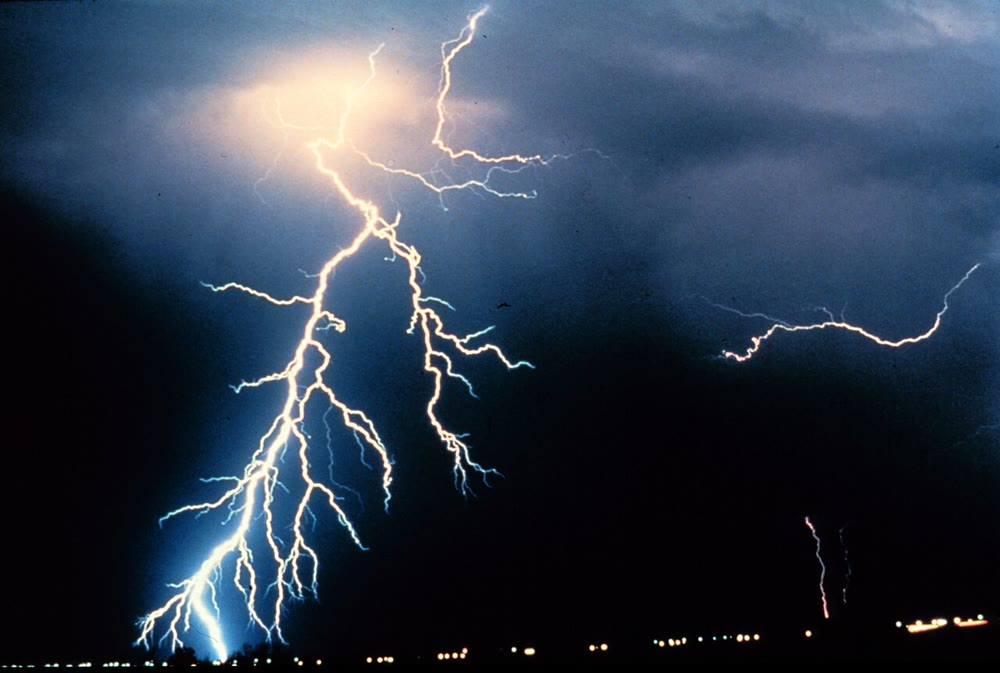
\includegraphics[width=0.62\linewidth]{images/book2/g10-noaa-lightning.jpg}

{\small 夜间\omterm{def:g10:storms-and-cyclones:thunderstorm}{雷暴}中的\omterm{def:g10:storms-and-cyclones:lightning}{闪电}，包括云与云之间的，以及从云到地面的，
照片：C.~Clark，NOAA 国家强风暴实验室
（公有领域）。}
\end{omfigure}

卫星统计全球的闪光，发现每年约有
14 亿次\omterm{def:g10:storms-and-cyclones:lightning}{闪电}，即每秒 44 次。
% ledger: christian:flash-rate

\begin{method}[由闪电与雷声的间隔估算风暴距离]\label{met:g10:storms-and-cyclones:distance}
\begin{enumerate}
  \item 闪光几乎瞬时到达；雷声
        以声速传播，约为 \qty{343}{m/s}，
        在气温 \qty{20}{\degreeCelsius} 时。
  \item 数出\omterm{def:g10:storms-and-cyclones:lightning}{闪电}与雷声之间的秒数 $t$。
  \item 距离为 $343\,t$ 米，大约每
        三秒约 \qty{1}{km}。
\end{enumerate}
\end{method}
% ledger: const:R, earth:Mmol (speed of sound computed in figdata/grade-10/cyclones.py)

\section{龙卷风}

\begin{definition}[龙卷风]\label{def:g10:storms-and-cyclones:tornado}
\emph{龙卷风}\index{龙卷风}是与地面接触、剧烈旋转的空气柱，
自积雨云底部悬垂而下。
\end{definition}

最强的\omterm{def:g10:storms-and-cyclones:tornado}{龙卷风}来自\emph{超级单体}，这类\omterm{def:g10:storms-and-cyclones:thunderstorm}{雷暴}的
上升气流整体旋转。\omterm{def:g10:storms-and-cyclones:tornado}{龙卷风}小而短暂：通常直径为几
百米，持续数分钟，平均路径约
\qty{5.6}{km}。但\omterm{def:g10:storms-and-cyclones:tornado}{龙卷风}在地表的风力最强：一台
移动雷达测得距地面约 \qty{135}{m/s}（约 \qty{480}{km/h}）的
风速，测量的是 1999 年 5 月俄克拉荷马州的一次\omterm{def:g10:storms-and-cyclones:tornado}{龙卷风}。美国
\omterm{def:g10:storms-and-cyclones:tornado}{龙卷风}数量多于其他任何国家，每年约 1200 次；\omterm{def:g10:storms-and-cyclones:tornado}{龙卷风}频发的其他地区有
加拿大草原、孟加拉国、阿根廷北部
、巴西南部和英国。
% ledger: spc:tornado

\begin{omfigure}
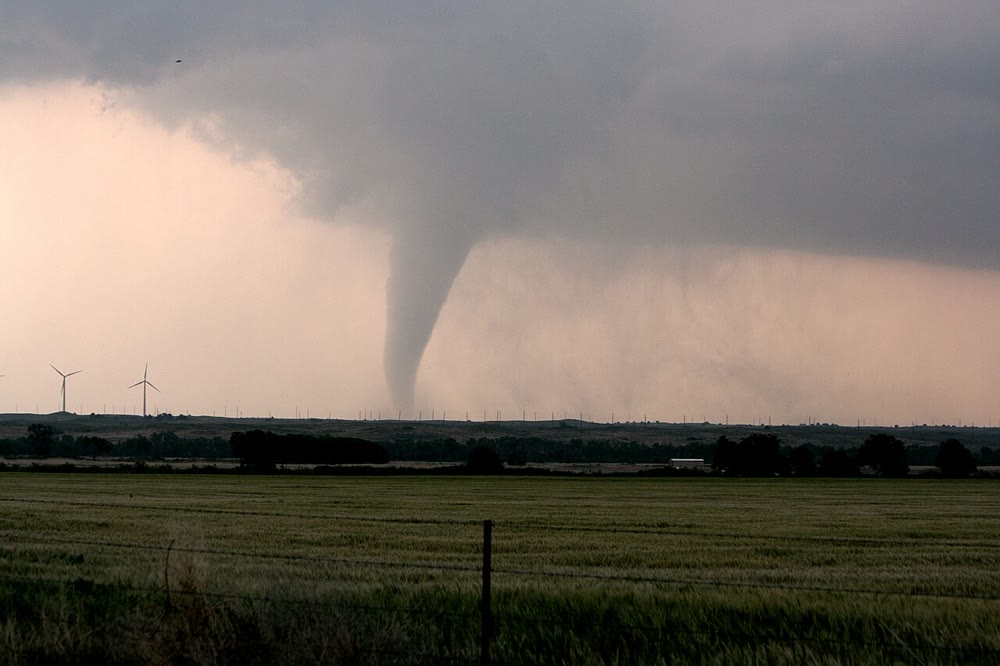
\includegraphics[width=0.62\linewidth]{images/book2/g10-noaa-tornado-kansas.jpg}

{\small 2008 年 5 月堪萨斯州平原上的一次\omterm{def:g10:storms-and-cyclones:tornado}{龙卷风}：漏斗云
自风暴云底部悬垂。照片：Sean Waugh，NOAA National Severe
Storms Laboratory（公有领域）。}
\end{omfigure}

\section{热带气旋}

\begin{definition}[热带气旋；风暴眼；眼墙]\label{def:g10:storms-and-cyclones:tropical-cyclone}
\emph{热带气旋}\index{热带气旋}是一种风暴，直径数
百千米，形成于温暖的热带海面上，围绕低压中心，
风沿螺旋状向中心汇聚，并伴有成带的
\omterm{def:g10:storms-and-cyclones:thunderstorm}{雷暴}。当其持续风速达到 \num{64}~节，约
\qty{119}{km/h}时，在大西洋和东太平洋称为飓风，在西太平洋称为台风，
在印度洋和南太平洋则简称为气旋。
其平静、几乎无云的中心是
\emph{风暴眼}\index{风暴眼}；其周围高耸的\omterm{def:g10:storms-and-cyclones:thunderstorm}{雷暴}环带，
即风力最强处，是\emph{眼墙}\index{眼墙}。
\end{definition}
% ledger: nhc:sshws

\begin{omfigure}
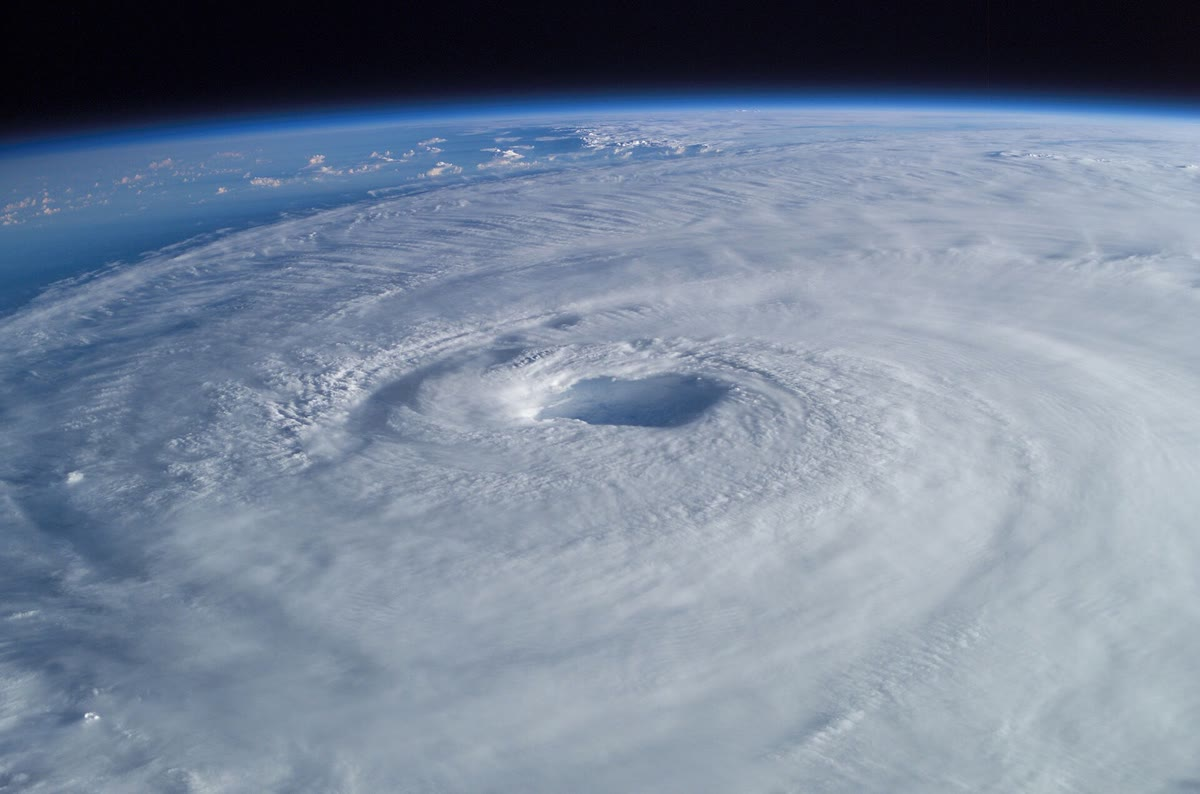
\includegraphics[width=0.78\linewidth]{images/book2/g10-nasa-hurricane-isabel.jpg}

{\small 飓风伊莎贝尔，2003 年 9 月 15 日，由国际空间站上的宇航员拍摄：
\omterm{def:g10:storms-and-cyclones:tropical-cyclone}{风暴眼}、\omterm{def:g10:storms-and-cyclones:tropical-cyclone}{眼墙}，以及围绕它们的螺旋状
云带。图像：Mike Trenchard，Earth Sciences and Image Analysis
Laboratory，NASA Johnson Space Center（公有领域）。}
\end{omfigure}

靠近海面处，湿润空气向低压中心
流入。地球自转使运动的空气在
北半球向右偏转：气流不再直接流向中心，而是
绕中心旋转，从上方看为逆时针（南半球为顺时针
）。靠近中心处，空气在\omterm{def:g10:storms-and-cyclones:tropical-cyclone}{眼墙}中上升、凝结，并
从风暴顶部流出。\omterm{def:g10:storms-and-cyclones:tropical-cyclone}{风暴眼}中少量空气下沉、增温
并变干：天空随之放晴。

\begin{omfigure}
\begin{tikzpicture}[font=\footnotesize, >={Stealth[length=2mm]}]
  \fill[omDef!25] (-6,-0.4) rectangle (6,0);
  \node[anchor=north, omDef!80!black] at (0,-0.05) {温暖海面};
  % rain bands
  \foreach \x/\h in {-5.0/1.6, -3.9/2.2, 3.9/2.2, 5.0/1.6}
    \fill[black!10, draw=black!45] (\x-0.35,0.4) -- (\x-0.3,\h) .. controls (\x-0.15,\h+0.35) and (\x+0.15,\h+0.35) .. (\x+0.3,\h) -- (\x+0.35,0.4) -- cycle;
  % eyewall towers and outflow canopy
  \fill[black!14, draw=black!50] (-2.4,0.4) -- (-2.5,4.0) -- (-5.8,4.3) -- (-5.6,4.7) -- (-1.0,4.9) -- (-0.75,4.0) -- (-0.8,0.4) -- cycle;
  \fill[black!14, draw=black!50] (2.4,0.4) -- (2.5,4.0) -- (5.8,4.3) -- (5.6,4.7) -- (1.0,4.9) -- (0.75,4.0) -- (0.8,0.4) -- cycle;
  % inflow, rise, outflow, eye subsidence
  \draw[->, thick, omThm!80!black] (-5.8,0.2) -- (-1.3,0.2) -- (-1.3,4.3) -- (-4.2,4.45);
  \draw[->, thick, omThm!80!black] (5.8,0.2) -- (1.3,0.2) -- (1.3,4.3) -- (4.2,4.45);
  \draw[->, thick, omDef!80!black] (0,4.3) -- (0,1.0);
  \node[anchor=south, align=center] at (0,5.0) {风暴眼：下沉 \\干燥空气};
  \node[anchor=south east, align=right] at (-2.6,4.95) {眼墙};
  \node[anchor=west, align=left] at (-5.95,2.9) {雨 \\带};
  \node[anchor=north, align=center] at (-3.6,0.15) {湿空气流入};
  \node[anchor=south east, align=right] at (5.8,4.95) {高空流出};
  % plan view
  \begin{scope}[shift={(8.4,2.3)}]
    \draw[black!40] (0,0) circle (1.7);
    \foreach \a in {0,90,180,270}
      \draw[->, thick, omThm!80!black, domain=0:200, samples=30, variable=\t]
        plot ({(1.6-0.0045*\t)*cos(\a+\t)}, {(1.6-0.0045*\t)*sin(\a+\t)});
    \fill[white, draw=black!50] (0,0) circle (0.22);
    \node[anchor=north, align=center] at (0,-1.8) {俯视 \\（北半球）};
  \end{scope}
\end{tikzpicture}

{\small \omterm{def:g10:storms-and-cyclones:tropical-cyclone}{热带气旋}剖面示意图（高度大幅夸大）：
湿润空气在温暖海面上流入，在\omterm{def:g10:storms-and-cyclones:tropical-cyclone}{眼墙}和
雨带中上升，并从顶部流出；\omterm{def:g10:storms-and-cyclones:tropical-cyclone}{风暴眼}中有少量空气下沉。
右图：北半球俯视时，流入气流绕中心
呈逆时针旋转。}
\end{omfigure}

\omterm{def:g10:storms-and-cyclones:tropical-cyclone}{热带气旋}需要温暖的海洋：表层水温至少约
\qty{27}{\degreeCelsius}，且水深约
\qty{46}{m} 深的范围内保持温暖。它们不会直接在赤道上形成，那里
地球自转不会使流入空气发生偏转：风暴须距赤道至少约
\qty{480}{km}，旋转才能开始。
% ledger: aoml:formation

\begin{omfigure}
\begin{tikzpicture}
\begin{axis}[ommap, width=\linewidth, xtick={-180,-120,...,180}, ytick={-60,-30,0,30,60},
  ymin=-70, ymax=70, unbounded coords=jump]
\addplot[fill=omLithAlluv, draw=black!45, line width=0.2pt] table {figdata/out/shared-geo-land.dat};
\addplot[omThm!70, line width=0.25pt] table {figdata/out/grade-10-cyclones-tracks.dat};
\addplot[only marks, mark=*, mark size=0.45pt, omDef!90!black] table {figdata/out/grade-10-cyclones-genesis.dat};
\addplot[black!45, dashed, domain=-180:180] {0};
\end{axis}
\end{tikzpicture}

{\small \omterm{def:g10:storms-and-cyclones:tropical-cyclone}{热带气旋}：2015--2024 年各季所有风暴的路径（红色），
以及 1980--2024 年各季每场风暴首次达到热带风暴强度的地点（蓝点）。
数据来源：IBTrACS v04r01，
NOAA 国家环境信息中心。}
\end{omfigure}
% ledger: data:b2-ibtracs (all statistics computed in figdata/grade-10/cyclones.py)

图中清楚地显示了这一规律。在 1980--2024 年的 3\,888 场风暴中，只有 24 场
在赤道 \qty{5}{\degree} 之内达到热带风暴强度。大多数风暴
形成于纬度 \qty{10}{\degree} 至 \qty{30}{\degree} 之间，
借信风向西漂移，并转向极地方向，
在寒冷海域中减弱。南大西洋水温较低、条件不利，
45 年间仅出现 3 场。平均每年约形成 87 个\omterm{def:g10:storms-and-cyclones:tropical-cyclone}{热带气旋}，
其中七成位于北半球，略超过半数
达到飓风强度。

\begin{proposition}[热带气旋的能量来源]\label{prop:g10:storms-and-cyclones:energy}
\omterm{def:g10:storms-and-cyclones:tropical-cyclone}{热带气旋}的能量取自温暖的海洋：海表蒸发吸收的\omterm{def:g10:earth-energy-budget:latent-heat}{潜热}，
在\omterm{def:g10:storms-and-cyclones:tropical-cyclone}{眼墙}与雨带中随蒸气凝结而释放。
一场平均强度的飓风以此方式释放
约 \qty{6e14}{W}；其中只有很小一部分，约 \qty{1.5e12}{W}，
转化为其风场的动能。
\end{proposition}
% ledger: aoml:energy

\begin{proof}[说明]
一场平均强度的飓风每天降雨 \qty{1.5}{cm}，覆盖半径为
\qty{665}{km} 的圆形区域，面积为 $\pi \times (665\,000)^2 \approx
\qty{1.39e12}{m^2}$：每天约 \qty{2.1e10}{m^3}，即 \qty{2.1e13}{kg} 的水。
每千克凝结的水释放约 \qty{2.5}{MJ}：$2.1\times10^{13}
\times 2.5\times10^6 \approx \qty{5.2e19}{J}$ 每天，即
$5.2\times10^{19}/86\,400 \approx \qty{6.0e14}{W}$。风的功率
由实测风场估算，数据取自同一来源。
\end{proof}

风暴如同一台热机运转：热量在温暖的海表被吸收，
在寒冷的高空被放出，部分温差转化为
风的运动。这正是\omterm{def:g10:storms-and-cyclones:tropical-cyclone}{热带气旋}移入陆地
或冷水上空时迅速减弱的原因：它失去了
蒸发水分的来源。

\section{强度、风与风暴潮}

\begin{definition}[萨菲尔–辛普森等级]\label{def:g10:storms-and-cyclones:scale}
\emph{萨菲尔–辛普森等级}\index{萨菲尔–辛普森等级}按最大持续风速将飓风
分为五个等级；
3 至 5 级的飓风为\emph{强飓风}。
\end{definition}

\begin{center}
\small
\begin{tabular}{cccc}
\hline
等级 & 节 & \unit{m/s} & \unit{km/h} \\
\hline
1 & 64--82 & 33--42 & 119--153 \\
2 & 83--95 & 43--49 & 154--177 \\
3 & 96--112 & 49--58 & 178--208 \\
4 & 113--136 & 58--70 & 209--251 \\
5 & 137 或以上 & 70 或以上 & 252 或以上 \\
\hline
\end{tabular}
\end{center}
% ledger: nhc:sshws (m/s converted with 1 knot = 1852/3600 m/s)

中心的气压越低，周围吹拂的风就越强，
这是因为中心与外界之间的气压差
驱动空气向内流动。

\begin{omfigure}
\begin{tikzpicture}
\begin{axis}[omrecord, width=0.86\linewidth, height=6.2cm, xmin=15, xmax=100,
  ymin=860, ymax=1015, xlabel={最大持续风速（\unit{m/s}）},
  ylabel={最低中心气压（\unit{hPa}）},
  tick label style={font=\small}, label style={font=\small}]
\foreach \w in {32.92, 42.70, 49.39, 58.13, 70.48}
  \edef\temp{\noexpand\draw[black!55, densely dashed] (axis cs:\w,860) -- (axis cs:\w,1015);}\temp
\addplot[only marks, mark=*, mark size=0.6pt, omDef!80!black, opacity=0.6] table[x=wind_ms, y=pmin_hpa] {figdata/out/grade-10-cyclones-scatter.dat};
\addplot[omThm!85!black, thick] table[x=wind_ms, y=pmin_hpa] {figdata/out/grade-10-cyclones-fit.dat};
\node[font=\scriptsize, black!60] at (axis cs:37.8,1008) {1};
\node[font=\scriptsize, black!60] at (axis cs:46.0,1008) {2};
\node[font=\scriptsize, black!60] at (axis cs:53.8,1008) {3};
\node[font=\scriptsize, black!60] at (axis cs:64.3,1008) {4};
\node[font=\scriptsize, black!60] at (axis cs:76,1008) {5};
\end{axis}
\end{tikzpicture}

{\small 每个点代表 2000--2024 年各季中的一个\omterm{def:g10:storms-and-cyclones:tropical-cyclone}{热带气旋}的
最强持续风速与最低中心气压。这条线是最佳直线拟合：风速每增加
一米每秒，中心气压约降低 \qty{1.6}{hPa}。灰色虚线为
\omterm{def:g10:storms-and-cyclones:scale}{萨菲尔–辛普森等级}的界线（编号
标于顶部）。数据来源：IBTrACS v04r01，NOAA NCEI。}
\end{omfigure}
% ledger: data:b2-ibtracs, nhc:sshws (fit computed in figdata/grade-10/cyclones.py)

档案中 1980--2024 年风暴的纪录属于飓风
帕特丽夏，2015 年 10 月位于墨西哥太平洋沿岸：持续风速
达 185 节，约 \qty{95}{m/s}，中心气压为 \qty{872}{hPa}。
% ledger: data:b2-ibtracs

\begin{definition}[风暴潮]\label{def:g10:storms-and-cyclones:storm-surge}
\emph{风暴潮}\index{风暴潮}是指海面高出其
正常水位的部分（不计潮汐），由风暴引起：风将海水向岸边推积，
低气压使风暴正下方的海面隆起。
\end{definition}

\begin{proposition}[气压隆起]\label{prop:g10:storms-and-cyclones:bulge}
若某风暴的中心气压比其外界低 $\Delta p$ 百帕，
则海面约升高 $\Delta p$ 厘米。
\end{proposition}

\begin{proof}
在远低于海面处，风暴下方与外部的压强必须相同，
否则海水将发生流动。风暴上方的空气重量
减少了 $\Delta p$；高度为 $h$ 的海水柱可以补偿这一差值，条件是
$\rho g h = \Delta p$。取 $\Delta p = \qty{1}{hPa} = \qty{100}{Pa}$，
$\rho = \qty{1025}{kg/m^3}$，$g = \qty{9.81}{m/s^2}$，则 $h = 100/(1025
\times 9.81) \approx \qty{0.0099}{m}$，约为 \qty{1}{cm}。
\end{proof}
% ledger: noaa:seawater-1025, nasa:aquarius-density, const:gn

对大多数\omterm{def:g10:storms-and-cyclones:storm-surge}{风暴潮}而言，隆起只占较小部分：中心气压为
\qty{920}{hPa}、比外界低 \qty{90}{hPa} 时，隆起高度约为
\qty{0.9}{m}。其余部分由风完成，风将海水推向海岸，
尤其是在宽阔而浅平的海底上方。若恰逢高潮到达，\omterm{def:g10:storms-and-cyclones:storm-surge}{风暴潮}
可达数米，可使低海岸被淹没，远及内陆。

\begin{omfigure}
\begin{tikzpicture}[font=\footnotesize, >={Stealth[length=2mm]}]
  \def\surf{(0,0) .. controls (1.5,0) and (2.2,0.5) .. (3.0,0.5) .. controls (3.8,0.5) and (4.6,0.4) .. (5.6,0.5) .. controls (7.2,0.65) and (8.8,1.0) .. (10.25,1.3)}
  \fill[omDef!20] (0,-1.6) -- \surf -- (8.8,-1.6) -- cycle;
  \draw[thick, omDef!80!black] \surf;
  \draw[black!50, dashed] (0,0) -- (9.6,0);
  \node[anchor=north west, black!60] at (0.1,-0.05) {正常海平面};
  \fill[omExo!30, draw=black!60] (8.8,-1.6) -- (10.4,1.6) -- (12.4,1.7) -- (12.4,-1.6) -- cycle;
  \foreach \x in {10.9,11.7} \draw[fill=white, draw=black!60] (\x,1.63) rectangle (\x+0.45,2.03) (\x-0.05,2.03) -- (\x+0.225,2.28) -- (\x+0.5,2.03);
  \draw[<->, omThm!80!black] (3.0,0) -- (3.0,0.5);
  \node[anchor=south east, omThm!80!black, align=right] at (2.8,0.6) {低压下的 \\隆起};
  \draw[<->, omThm!80!black] (9.4,0) -- (9.4,1.12);
  \node[anchor=south, omThm!80!black, align=center] at (8.9,1.75) {风壅水 \\推向海岸};
  \foreach \y in {2.9,3.4} \draw[->, thick, black!60] (4.0,\y) -- (6.4,\y);
  \node[anchor=south] at (5.2,3.45) {向岸风};
  \node[anchor=south, align=center] at (3.0,1.9) {风暴 \\中心};
  \draw[black!40] (3.0,1.9) -- (3.0,0.65);
\end{tikzpicture}

{\small \omterm{def:g10:storms-and-cyclones:storm-surge}{风暴潮}示意图（高度大幅夸大）：海面约升高
\qty{1}{cm}，对应风暴下方每百帕的低压，
向岸风则将海水推积在海岸。}
\end{omfigure}

\begin{omfigure}
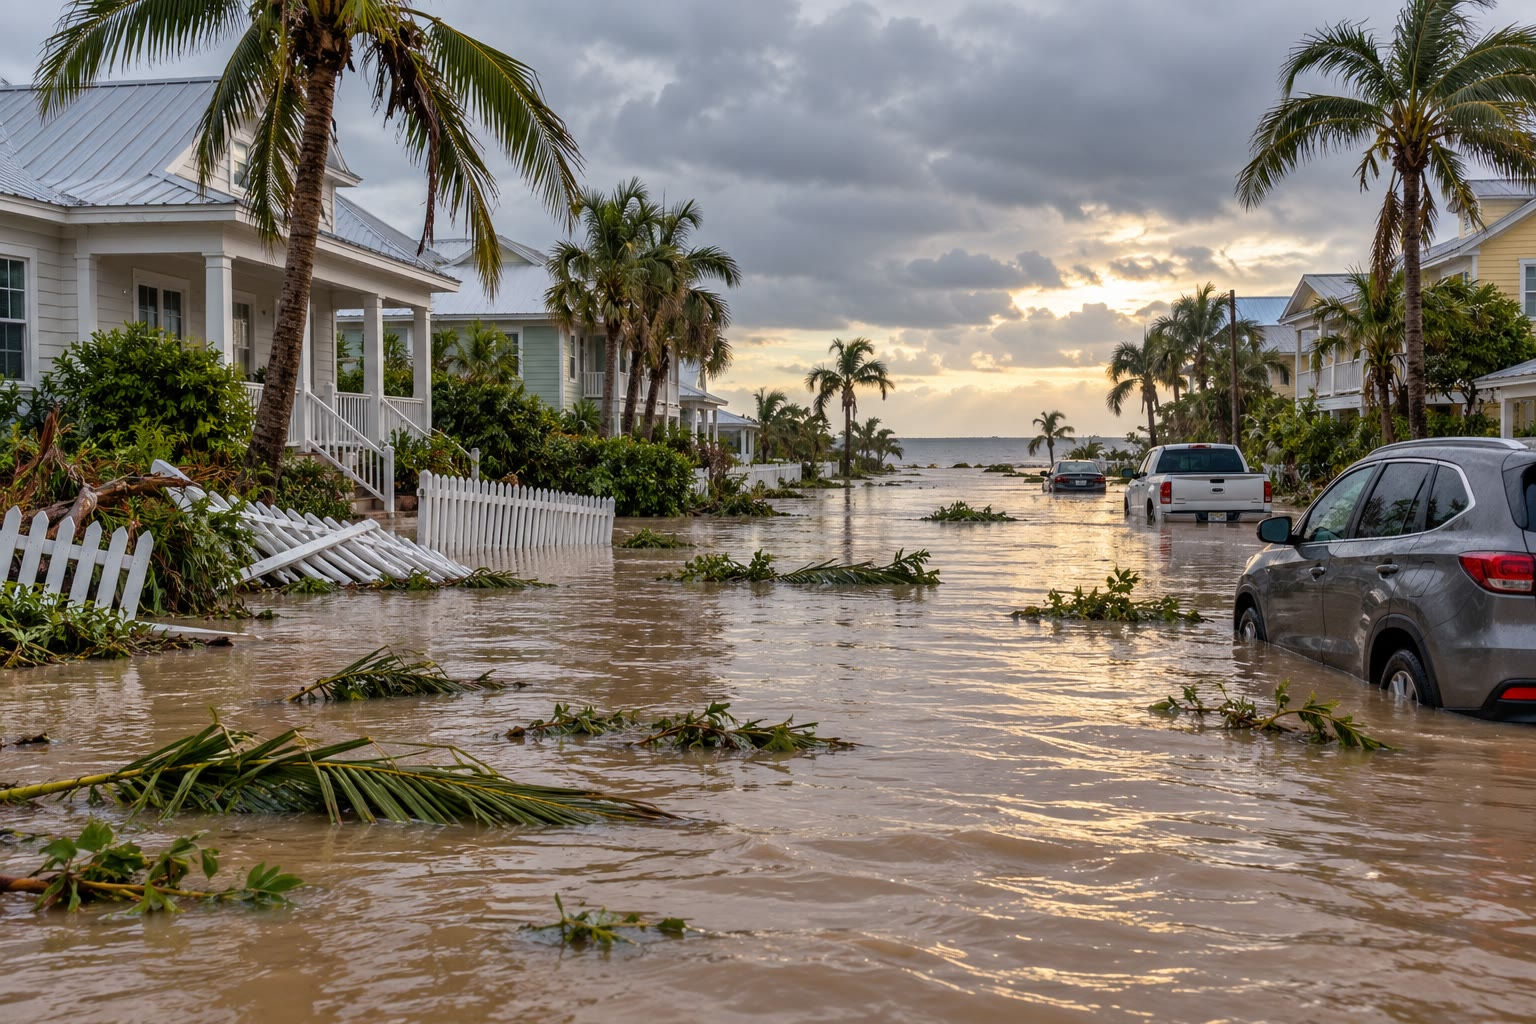
\includegraphics[width=0.7\linewidth]{images/book2/ai/g10-flooded-street.jpg}

{\small \omterm{def:g10:storms-and-cyclones:storm-surge}{风暴潮}过后次日清晨的一条沿海街道：海水、
折断的棕榈树和破损的围栏。}
\end{omfigure}

\section{练习}

\begin{exercise}[$\star$]\label{exo:g10:storms-and-cyclones:1}
给出\omterm{def:g10:storms-and-cyclones:thunderstorm}{雷暴}和\omterm{def:g10:storms-and-cyclones:lightning}{闪电}的定义。雷声是由什么产生的？
\end{exercise}

\begin{exercise}[$\star$]\label{exo:g10:storms-and-cyclones:2}
给出\omterm{def:g10:storms-and-cyclones:tropical-cyclone}{热带气旋}、其\omterm{def:g10:storms-and-cyclones:tropical-cyclone}{风暴眼}和\omterm{def:g10:storms-and-cyclones:tropical-cyclone}{眼墙}的定义。其风速
最大处位于何处？
\end{exercise}

\begin{exercise}[$\star$]\label{exo:g10:storms-and-cyclones:3}
在\omterm{def:g10:storms-and-cyclones:scale}{萨菲尔–辛普森等级}中，持续风速为
\num{70}~节、\num{120}~节和\num{140}~节的飓风分别属于哪一等级？
其中哪些是大飓风？
\end{exercise}

\begin{exercise}[$\star$]\label{exo:g10:storms-and-cyclones:4}
你数出\omterm{def:g10:storms-and-cyclones:lightning}{闪电}与雷声之间相隔 \num{9}~秒，随后
下一次\omterm{def:g10:storms-and-cyclones:lightning}{闪电}的间隔为 \num{15}~秒。两次\omterm{def:g10:storms-and-cyclones:lightning}{闪电}各距离
多远？风暴是否正在靠近？
\end{exercise}

\begin{exercise}[$\star$]\label{exo:g10:storms-and-cyclones:5}
解释为什么田野中孤立的一棵树
在\omterm{def:g10:storms-and-cyclones:thunderstorm}{雷暴}中是危险的避身处，并说明应改到何处。
\end{exercise}

\begin{exercise}[$\star\star$]\label{exo:g10:storms-and-cyclones:6}
一节即每小时 \qty{1852}{m}。将 \num{64}~节和
\num{137}~节分别换算为 \unit{m/s} 和 \unit{km/h}。
\end{exercise}

\begin{exercise}[$\star\star$]\label{exo:g10:storms-and-cyclones:7}
地球上每秒发生 44 次\omterm{def:g10:storms-and-cyclones:lightning}{闪电}。这相当于一天内
和一年内各有多少次\omterm{def:g10:storms-and-cyclones:lightning}{闪电}？
\end{exercise}

\begin{exercise}[$\star\star$]\label{exo:g10:storms-and-cyclones:8}
某飓风中心气压为 \qty{935}{hPa}，外界气压为
\qty{1010}{hPa}。求其下方海面隆起的高度为多少？
\end{exercise}

\begin{exercise}[$\star\star$]\label{exo:g10:storms-and-cyclones:9}
利用路径图，描述\omterm{def:g10:storms-and-cyclones:tropical-cyclone}{热带气旋}形成的位置，以及
形成后的移动路径。为什么\omterm{def:g10:storms-and-cyclones:tropical-cyclone}{热带气旋}在赤道上本身不出现？
\end{exercise}

\begin{exercise}[$\star\star$]\label{exo:g10:storms-and-cyclones:10}
气压–风速图中的直线为 $p \approx 1031 - 1.56\,v$，
（$p$ 的单位为 \unit{hPa}，$v$ 的单位为 \unit{m/s}）。该直线给出的
5 级下限 \qty{70}{m/s} 对应的中心气压为多少？风速为
\qty{40}{m/s} 的风暴，其中心气压又为多少？
\end{exercise}

\begin{exercise}[$\star\star$]\label{exo:g10:storms-and-cyclones:11}
说明\omterm{def:g10:storms-and-cyclones:tropical-cyclone}{热带气旋}为何在移至陆地上后迅速减弱，
以及为什么它在冷水上也会减弱。
\end{exercise}

\begin{exercise}[$\star\star\star$]\label{exo:g10:storms-and-cyclones:12}
空气中的声速为 $\sqrt{1.4\,R\,T/M}$，其中 $R =
\qty{8.314}{J.mol^{-1}.K^{-1}}$，$T$ 以开尔文为单位，且 $M =
\qty{0.02897}{kg/mol}$。求其在 \qty{0}{\degreeCelsius} 和
\qty{30}{\degreeCelsius} 时的值。若延迟为 \qty{9}{s}，则两段距离相差多少？
“\qty{3}{s} 每千米”这一规则是否足够精确？
\end{exercise}

\begin{exercise}[$\star\star\star$]\label{exo:g10:storms-and-cyclones:13}
一场飓风登陆，沿岸测得\omterm{def:g10:storms-and-cyclones:storm-surge}{风暴潮}高 \qty{4.0}{m}。该飓风中心气压为
\qty{940}{hPa}，外界气压为 \qty{1010}{hPa}。
\omterm{def:g10:storms-and-cyclones:storm-surge}{风暴潮}中有多少是由气压凸起引起的，多少是由风引起的？
若其在高潮时到达，高潮位比平均海平面高 \qty{1.5}{m}，
则海水会上升到比平均海平面高多少？
\end{exercise}

\begin{exercise}[$\star\star\star$]\label{exo:g10:storms-and-cyclones:14}
一次\omterm{def:g10:storms-and-cyclones:tornado}{龙卷风}中，距轴线 \qty{100}{m} 处风速为 \qty{90}{m/s}；
一次飓风中，距中心 \qty{30}{km} 的\omterm{def:g10:storms-and-cyclones:tropical-cyclone}{眼墙}处风速为 \qty{60}{m/s}。
空气绕行一周各需多长时间？请加以比较。
\end{exercise}

\begin{exercise}[$\star\star\star$]\label{exo:g10:storms-and-cyclones:15}
1980--2024 年间的 3\,888 个\omterm{def:g10:storms-and-cyclones:tropical-cyclone}{热带气旋}中，有 24 个达到热带风暴强度，
发生于距赤道 \qty{5}{\degree} 以内，414 个发生于
\qty{10}{\degree} 以内，121 个发生于 \qty{30}{\degree} 以外。计算这三个
百分比。赤道两侧 \qty{5}{\degree} 以内的带状区域约占
地球表面的 \qty{9}{\percent}：若纬度无关，应预期
该区域内占比应为多少？由此可得出什么结论？
\end{exercise}

\section{问题：飓风的热机}

\begin{problem}[{周末问题——从一天的降雨到风的
功率}]
\label{pb:g10:storms-and-cyclones:1}
% ledger: aoml:energy, nist:water-latent, earth:Rmean, ipcc:budget-toa (all results computed in figdata/grade-10/cyclones.py or from the rounded data below)
一次平均飓风，每天在半径为
\qty{665}{km} 的圆形区域上降雨 \qty{1.5}{cm}。取\omterm{def:g10:earth-energy-budget:latent-heat}{潜热}为 \qty{2.5}{MJ/kg}，水的密度为
\qty{1000}{kg/m^3}，一天取 \qty{86400}{s}，以及平均飓风的
风功率 \qty{1.5e12}{W}。

\medskip
\noindent\textbf{第一部分——一天的降雨。}
\begin{enumerate}
  \item 计算该圆的面积。
  \item 计算该圆形区域一天内降雨的体积。
  \item 将其换算为立方千米。
  \item 计算其质量。
\end{enumerate}

\medskip
\noindent\textbf{第二部分——释放的热量。}
\begin{enumerate}[resume]
  \item 计算这些水凝结时一天内释放的
        \omterm{def:g10:earth-energy-budget:latent-heat}{潜热}。
  \item 将其换算为功率。
  \item 全球约吸收 \qty{1.22e17}{W} 的太阳辐射
        （见\cref{ch:g10:earth-energy-budget}），一次飓风释放的
        热量占其中的多大比例？
  \item 平均吸收的太阳辐射为 \qty{240}{W/m^2}。计算
        风暴所占区域吸收的太阳辐射，并将其与
        风暴的\omterm{def:g10:earth-energy-budget:latent-heat}{潜热}相比较。
  \item 这一比较说明，风暴的能量是从何处
        汇集而来的？
\end{enumerate}

\medskip
\noindent\textbf{第三部分——水从何而来。}
\begin{enumerate}[resume]
  \item 为了维持这场降雨，每天必须蒸发多少质量的水？
  \item 地球表面的平均蒸发携带的热量为
        \qty{82}{W/m^2}。以平均蒸发提供风暴\omterm{def:g10:earth-energy-budget:latent-heat}{潜热}，需要多大面积？
        并与风暴自身的面积相比较。
  \item 利用\cref{ch:g10:why-clouds-form}中的\omterm{def:g10:why-clouds-form:humidity}{饱和}含水量表，
        比较\omterm{def:g10:why-clouds-form:humidity}{饱和}空气在 \qty{28}{\degreeCelsius} 和
        \qty{20}{\degreeCelsius} 时所含的水量。
  \item 说明\omterm{def:g10:storms-and-cyclones:tropical-cyclone}{热带气旋}为何只在温暖的海面上形成。
  \item 说明\omterm{def:g10:storms-and-cyclones:tropical-cyclone}{热带气旋}为何在陆地上减弱。
\end{enumerate}

\medskip
\noindent\textbf{第四部分——风。}
\begin{enumerate}[resume]
  \item 计算一天内赋予风的动能。
  \item 将 3 级的下限 \num{96}~节换算为
        \unit{m/s}（\num{1}~节 = \qty{1852}{m/h}）。
  \item 海面附近空气的密度约为
        \qty{1.16}{kg/m^3}。计算一立方米以该速度运动的
        空气的动能。
  \item 将一天内凝结释放的\omterm{def:g10:earth-energy-budget:latent-heat}{潜热}，与一天内
        风所具有的能量相比较。
  \item 释放的其余热量去向何处？
  \item 凝结释放的热量中，有多大比例转化为风？
\end{enumerate}
\end{problem}
